\documentclass[a4paper,12pt]{article}

\usepackage{url}
\usepackage{epsfig}
\usepackage{graphics}
\usepackage{fancyhdr}
\usepackage{indentfirst}
\usepackage{hyperref}
\usepackage{amsmath}
\usepackage{algorithm}
\usepackage{algpseudocode}

\graphicspath{{pictures/}}

\title{A Comparison of N-gram and Hidden Markov Model Text Generators}
\author{\hspace*{-0.5cm}\begin{tabular}{cccc}
Akash Kumar Dhaka & Dario Vidas & Stefan Annell \\
1990-02-26 & 1992-06-24 & 1987-09-30 \\
akashd@kth.se & vidas@kth.se & steann@kth.se \\

\includegraphics[width=0.13\linewidth]{akash} & 

\includegraphics[width=0.13\linewidth]{dario} & 
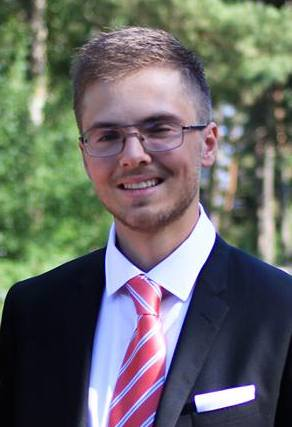
\includegraphics[width=0.13\linewidth]{stefan} 
\end{tabular}} 
% Normally there will not be any pictures but we want
% these so that we can connect faces to names in the course
% We also want birthdates so that we can tell people with the same
% name apart
\date{}

\pagestyle{fancy}
\setlength{\headheight}{15pt}
\fancyhf{}
\lhead{DD2380 ai14} % DO NOT REMOVE!!!!
\rhead{A.K. Dhaka, D. Vidas, S. Annell} %% UPDATE WITH YOUR NAMES

\begin{document}

\nocite{*}

\maketitle
\thispagestyle{fancy}

\begin{abstract}
Natural Language Generation (NLG) is a Natural Language Processing (NLP) task of
generating natural language. The problem is well known and well researched, but
the field is far from being fully explored. In this paper, we propose an idea of
building a text generator based on Hidden Markov Model (HMM). HMM allows us to
append words in a sentence that depend on a whole sequence until that point,
unlike other methods, such as n-gram, which use only a certain number of words
to predict the next one. We implemented three different types of HMM models for
generation- unsupervised, supervised and chunked supervised. Three different evaluators 
were used for comparing the performance of the generators with human written-sentences. 
Their respective performace suggested to us that HMM generators work better than 
trigram generator over a small corpus and gives much more random texts whereas 
the latter generates better sentences when fed in with a large corpus.

\end{abstract}



\clearpage

%%%%%%%%%%%%%%%%%%%%%%%%%%%%%%%%%%%%%%%%%%%%%%%%%%%%%%%%%%%%%
%%%%%%%%%%%%%%%%%%%%%%%%%%%%%%%%%%%%%%%%%%%%%%%%%%%%%%%%%%%%%
\section{Introduction}
\label{sec:intro}
Natural Language Generation(NLG) is the field of generating natural language for
a computer from a knowledge base or some information that the system can
understand. Some fields where the NLG is being applied are weather
forecast generation, summarize statistical data extracted from a database and
describing chains of reasoning performed by a system~\cite{nlgsystem01}.

This paper is about designing, implementing and comparing different methods of
generating random sentences when fed in by a specific corpus. The generated 
sentences should be as correct as possible grammatically and semantically,
which means that Natural Language Processing (NLP) needs to be implemented
for building the corpus and tagging / structuring the words, allowing our system
to form sentences that are meaningful and semantically as correct as possible.
The corpora used were of different sizes to test our system properly.

This is very interesting field of research and a good topic to study because it
incorporates several complicated tasks that are useful in wide variety of
applications. First of all, it is very difficult for a computer to understand
the content of a text, although there has been a lot of work done in this field. 
It is also hard for a computer to construct sentences that are correct
semantically because of the complexity of a natural languages, such as English
as mentioned in \cite{nlgScratch}. The evaluation of how correct a sentence is 
also very challenging and a field in its own. Furthermore, the 
aggravating circumstance that the language (both dictionary and the grammar)
is continuously evolving, makes it even harder to define a specific set of rules 
that apply all the time, considering that our datasets are written by numerous
authors and in different time instants. NLG systems broadly have three
subcomponents: text planning, sentence planning and surface realisation.
In text planning, content and target of the text are determined. During sentence
planning, syntactic and lexical means are ascertained whereas in realisation, 
actual words are strung together to give form to the basic structure which comes out
of sentence planning. 

It is also preferred if the results are benchmarked in some systematical way,
either manually (which is not preferred), semi-manually where the system might
give suggestions and the operator help the computer or it is done completely
automated (which is also quite hard).


\subsection{Contribution}
It is very hard for a computer to communicate with a human since the language is
very complex and it is hard to replicate and the language is one of the big
borders between computers and humans which makes this field of research very
interesting. The method that we are presenting is a new and interesting way to
generate text focused on a topic using Hidden Markov Models (HMM). We used
three variants of HMM for this taks- unsupervised HMM, supervised HMM and 
chunked supervised HMM. We also generated sentenced by trigrams and evaluated
the performance of all the generators with human written sentences using evaluators.

\subsection{Outline}
In Section~\ref{sec:relwork} previous work is recognized and the papers we have
researched to support our work is presented. Section~\ref{sec:method} contains
an overview on how we are going to solve the problem, and why we are choosing a
specific method and also how we are implementing the system. The result of the
implementation is presented in Section~\ref{sec:exps} and the whole paper is
summarized and concluded in Section~\ref{sec:summary}.

%%%%%%%%%%%%%%%%%%%%%%%%%%%%%%%%%%%%%%%%%%%%%%%%%%%%%%%%%%%%%
%%%%%%%%%%%%%%%%%%%%%%%%%%%%%%%%%%%%%%%%%%%%%%%%%%%%%%%%%%%%%
\section{Related work}
\label{sec:relwork}

The field of NLG and NLP are two very large fields that are subfields of
artificial intelligence and computational linguistics. A lot of research has
been done in these fields, although the fields are far from fully explored. Some
of the earliest work in this field was performed in the 1970's by people like
Goldman and Davey, where they helped to define the main problems in NLG 
as explained in \cite[p.~19-20]{buildingNLG}, where they also mention that NLG
started to be researched allot during 1980's by people like McKeown and Appelt
that had a big impact on how the subsequent research was going to be performed on NLG.
The field had a big increase in the 1990's where a lot of real-world applications were made,
like the weather forecast system FOG.

The paper Building Applied Natural Language Generation
Systems~\cite{nlgsystem01} is about the architecture and how to structure a
NLG system when designing it. They describe six main tasks that needs to be
performed when generating a text; content determination, discourse planning,
sentence aggregation, lexicalization, referring expression generation and
linguistic realisation. They also discuss the sub components the system
needs to design and the algorithms, using which the different subproblems can be
solved. The main use of this paper is the structure of the generation part of
the system, but also suggestions and pointers on how the arising problems can be
solved.

Usage of HMMs in text generation is mentioned in~\cite{hmmnlg} where the model
is used in a task-oriented environment. Authors describe HMM generation process
to be very similar to POS (part of speech) tagging. States represent words, and
state sequences, word phrases. The model is designed from the corpus data
using ABL algorithm and it learns using the Baum-Welch algorithm.

The paper Shallow Parsing Using Specialized HMMs~\cite{hmmchunk} uses the technique
of chunking for parsing a sentence, which we have used in one of our HMM generator.

These papers  ~\cite{poseval} ~\cite{bleueval} researched some different methods for evaluating Natural Language Generation systems, by comparing automated methods and human evaluation methods. Where  ~\cite{bleueval} propose methods like Bleu, NIST and Rogue which looks at the words of the generated sentence, and compares it to a reference. ~\cite{poseval} Suggests a pos tagging method, that breaks up the sentences into POS tags, and compares it to a big reference corpus.
They both discuss the pros and cons of the evaluation systems and suggests that a combination of automated methods should be used, since the different automated methods covers different parts of the text.

%%%%%%%%%%%%%%%%%%%%%%%%%%%%%%%%%%%%%%%%%%%%%%%%%%%%%%%%%%%%%
%%%%%%%%%%%%%%%%%%%%%%%%%%%%%%%%%%%%%%%%%%%%%%%%%%%%%%%%%%%%%
\section{Hidden Markov Model}
\label{sec:method}

\subsection{N-gram}
n-gram models have been used for the task of NLG~\cite{nlgngram}. n-gram models use the
statistical property of co-occurrances to calculate the most likely word to
appear given previous (n-1) grams. We have used trigrams as one of the generation techniques,
But there are  also some problems with n-gram models. One of them 
is of the sparse data combinations as n becomes greater. The other problem which will be 
verified in the results section is that of non-randomness. Trigram tends to 
pick full sentences out of the corpus and that is where HMMs perform much
better over trigrams. This problem with ngrams gets aggravated if the training
corpus is small in size. 


\subsection{Hidden Markov Models}
Hidden Markov Model (HMM) is a tool for modelling time series data.
It can be presented as a dynamic Bayesian network. In HMM, ``hidden''
stands for the states which are not directly visible to the observer~\cite{hmm}.
A certain HMM is fully defined by its:
\begin{itemize}
  \item transition matrix $A$,
  \item emission matrix $B$,
  \item initial state probability distribution $\pi$.
\end{itemize}

We propose to use HMMs for the surface generalisation task. HMMs have been used
with very good results in the fields of speech recognition and also in NLU
(Natural Language Understanding)~\cite{hmmsr}. The idea of HMM in this work is
to do something similar to the inverse of what POS Tagging does. In POS
Tagging, an input string of words is mapped to a hidden sequence of semantic POS
tags. The POS Tags then can serve as the hidden states in the HMM model and the
words as the observations. The algorithm used for generating text with HMMs is
described by Algorithm~\ref{alg:hmm}.

In our work, we have used three types of HMMs for the text generation:
\textit{supervised, supervised with text chunking and unsupervised}.

\begin{algorithm}
\caption{HMM Text Generation Algorithm}
\label{alg:hmm}
\begin{algorithmic}[1]
	\State $sequence \gets \emptyset$
	\State $state \gets \Call{pickRandomState}$
	\Repeat
		\State $emission \gets \Call{generateEmission}{state}$
		\State $sequence \gets \Call{append}{sequence, emission}$
		\State $state \gets \Call{stateTransition}{state}$
	\Until{enough} \\
	\Call{output}{sequence}
\end{algorithmic}
\end{algorithm}

\subsubsection{Supervised HMMs}
\label{sec:suphmm}
In the supervised HMMs, the POS tags are used as the states and the words and
punctuation of the corpus are treated as the emissions. NLTK's~\footnote{Natural
Language Toolkit - Open source library for NLG written in python} default POS Tagger was
used for evaluating the POS tags in a sentence. The state-transition matrix and
emission matrix are then computed with them, using the supervised learning
algorithm. The algorithm is purely statistical and is described by the
following equations:
\begin{align}
\label{eq:hmm}
A_{ij} = \frac{S_{ij}}{\sum_{k} S_{ik}} \qquad
B_{i}(w) = \frac{E_{i}(w)}{\sum_{w'} E_{i}(w')} \qquad
\pi_{i} = \frac{S_{i}}{\sum_{k} S_{k}}
\end{align}
where $S_{ij}$ is the number of occurrences of transitions from state $i$ to
state $j$, $E_{i}(w)$ is the number of occurrences of the observation $w$ in the
state $i$ and $S_{i}$ is the number of occurrences of state $i$. The
parameters of the HMM (matrix $A$, matrix $B$ and vector $\pi$) are easily
computed using the equations~\ref{eq:hmm}.

\subsubsection{Supervised HMMs with Text Chunking}
This type of HMM is an extension of a supervised HMM descibed in
section~\ref{sec:suphmm}. Text chunking is a method of grouping words in a
sentence, in a way that they produce semantical units. It has been successfully 
applied for the task of shallow parsing~\cite{hmmchunk}. The idea is to enrich the
observations with information on the parts(chunks) of a sentence like Noun phrase(NP)
and verb phrase(VP). For example, the sentence
\textit{``The quick brown fox jumps over the lazy dog.''} gets splitted into the
following chunks: \textit{``The quick brown fox'', ``jumps'', ``over'', ``a lazy
dog'', ``.''}. It can be clearly seen now that \textit{``The quick brown fox''}
is a single semantical unit.

In the chunked HMMs, we try to enrich the emissions with more
information about the semantics of a sentence and thus add chunk tags with POS
tags as hidden states. We also add chunks as emissions, which have previously
consisted of only words and punctuation. The learning algorithm is exactly the
same as the one used for the regular supervised HMMs.

\subsubsection{Unsupervised HMMs}
Unsupervised HMMs differ from supervised ones in several ways. The states are
implicit, the learner only knows the number of states but not what they
represent. The algorithm used for learning is Baum-Welch, which is a special
case of expectation maximization algorithm. Using this algorithm, we let the
learner find the patterns in the data and infer the states itself. The emissions
in unsupervised HMMs are the same as the ones in supervised HMMs.


\subsection {Performance measures for experiments}

As in other scientific fields, it is crucial to test how well our systems,
modules and algorithms work. This type of performance measure is called
evaluation. There are three techniques of evaluating NLG systems: task-based,
human ratings and metrics~\cite{evalnlg}. In our project we are going to use
metric evaluations.

Evaluation gives as an output the ``goodness'' of a sentence or a text. The
``goodness'' is defined by three characteristics: fluency, adequateness and
readability~\cite{evalmethods}. It is often a difficult task to assess each
characteristic.
Human ratings are based on opinions of individuals rating the given the given
text. These types of evaluations are subjective and hard to measure. But the
main advantage is the that the natural language is made for interactions between
people and we can evaluate texts more accurately than machines. In our project
we will spend a certain amount of time evaluating our models ourselves and with
the help of others to reduce the bias.

Metric evaluations are based on software evaluations of generated text. They are
more objective than human ratings, but also less reliable. Most evaluators
compare generated text with texts written by people to compute the score. In our
project, we used three evaluators- BLEU, Linguitic checker and POS sequence checker~\cite{autoeval}.
BLEU (Bilingual Evaluation Understudy) is an algorithm for evaluating the quality of a 
machine-translated text from one natural language to other. The way we have used it 
for our task is that, we compare the generated sentence with all the sentences of the
corpus in 4-grams which is considered the best number for evaluation ~\cite{bleueval}
 and then calculate the maximum score out of it.

For evaluating the grammatical correctness of the generated sentence, we used the
open source tool named LANGUAGE TOOL. This software is quite clean and robust. It gives 
all the possible errors and their description when it is fed with a sentence. The number 
of errors in a sentence per the number of words in a sentence can be used as a measure
for evaluating the grammatical correctness of a sentence.

The third test used for evaluation is the POS tag sequence checker. This measure 
gives us a good estimate of how correct the sentence is correct semantically. The idea
is that a good sentence will have a particular sequence of POS tags. So, the similarity
between a generated sentence is calculated with all the sentences of a corpus and the 
maximum score is taken as the final score. 

\subsection{Implementation}
\label{sec:impl}

We have used NLTK~\cite{nltk} very extensively. We used the built in brown
corpus and POS tagger trained on UPenn datasets. 
For the evaluation, the native implementation of BLEU in NLTK was used. 
For the linguistic checker evaluator, the open source tool LANGUAGE TOOL with a python
wrapper was used.

%%%%%%%%%%%%%%%%%%%%%%%%%%%%%%%%%%%%%%%%%%%%%%%%%%%%%%%%%%%%%
%%%%%%%%%%%%%%%%%%%%%%%%%%%%%%%%%%%%%%%%%%%%%%%%%%%%%%%%%%%%%
\section{Experimental results}
\label{sec:exps}

\subsection{Experimental setup}

We made two sets of tests with two different corpus as training data which were very different in length.
The longer corpus we used was a H.C. Andersen book, The Emperors new Cloths, which was about 60 000 words. 
The short corpus was information about zebras that was pulled from Wikipedia which was about 2000 words.
When performing the tests around 20 sentences were generated for each corpus with each of the four systems and also 20 human written sentences were produced. 
Then they were evaluated with the automated evaluation methods which generated a score for each of the systems.
The score of the human written sentences was used as a performance reference. Then the results were plotted and compared
towards each other and the manually generated scores.
\subsection{Experiment}
\begin{figure}
\centering
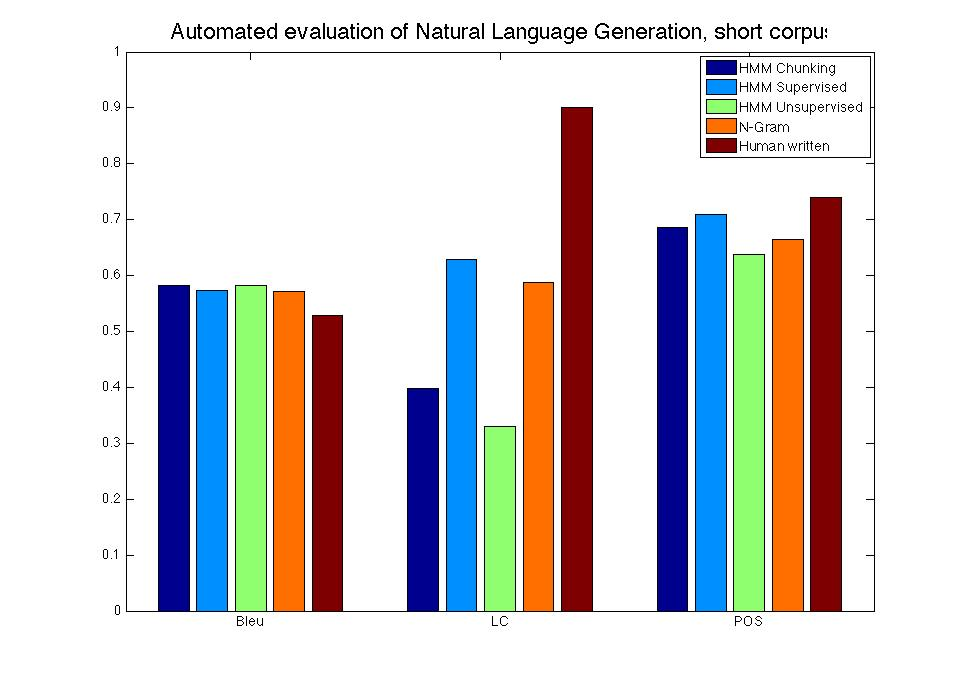
\includegraphics[width=0.8\linewidth]{resultsShort}
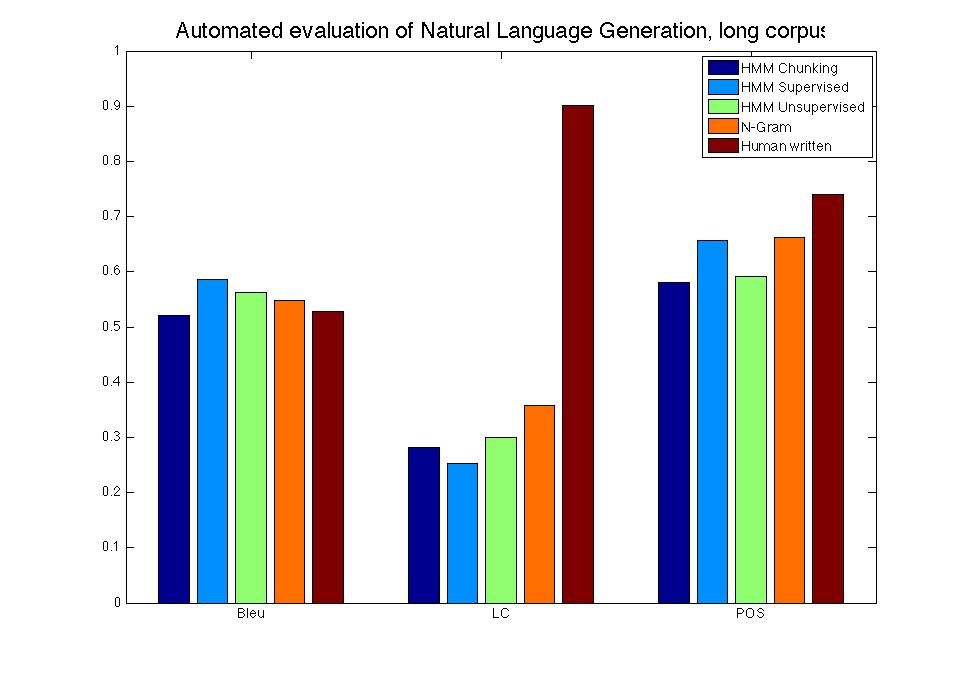
\includegraphics[width=0.8\linewidth]{results}
\caption{Experimental results when generating sentences with the four tested systems for a long corpus and a short corpus respectively, using the three automated evaluation methods, and comparing it to the human results.}
\label{fig:longresults}
\end{figure}

As seen from the Figure~\ref{fig:longresults} the Bleu results are all very close to the human results. Since human results are used as a
benchmark value on what score a good sentence should get and since all our results are close to the human results
we found that they are to unreliable  and because of this, we disregarded the Bleu score from our results.
As we can see the human generated sentences do not always have a score equal to 1 but close to it, which
highlights the shortcomings of the evaluators we have used and also because the evaluators have been trained on
different corpora.

In the long corpus from Figure~\ref{fig:longresults}, the trigrams performed the best since it received the highest LC and POS score, which co-relates with the
grammatical and the semantics of the sentence. The HMM systems were all pretty similar, but the Supervised HMM performed
a little bit better on the POS then the other systems.

The short corpus gave a lower score for trigrams and a higher score for all the HMM systems, where the supervised was the best.
Overall the score was higher and closer to the human score with a shorter corpus.
The results of the trigrams here is quite deceiving, since the sentences are not true random it is basically only a copy of the 
corpus. Which is also the nature of trigrams when dealing with a shorter corpus. So even tho the results look ok, the sentences
aren't very good since it is not random.

The chunking HMM system were introduced to increase the performance of the supervised HMM score. But even tho the
testing on the short corpus gives a better result then the long corpus the chunking HMM still performs worse then the 
supervised HMM.
A problem that we could see when generating sentences with all our HMM systems was that it generated way to many punctuations and citations.

%%%%%%%%%%%%%%%%%%%%%%%%%%%%%%%%%%%%%%%%%%%%%%%%%%%%%%%%%%%%%
%%%%%%%%%%%%%%%%%%%%%%%%%%%%%%%%%%%%%%%%%%%%%%%%%%%%%%%%%%%%%
\section{Summary and Conclusions}
We found that it is very hard to generate a sentence. When having a open sentence that's not constricted at all, 
the possible ways to build a sentence are almost endless. Using a story as a corpus and generating sentences 
is even more difficult as it needs to model the linguistic tools and there are much more degrees of freedom.
The Trigram system that we designed worked better then the HMM systems for a long corpus, but for the short corpus
the trigrams just copied whole sentences from the corpus thus performing very bad. 
The HMM got a better score for the shorter corpus probably because of the lesser occurrence of punctuation and citation marks.
One of the reasons why we didn't perform better could have been that we needed to tune the HMM's better and have more
testdata. And we also probably would need some kind of filter to be able to filter the data either that we input to the HMM's or
output from the HMM's.
When we tried to improve our HMM results by using chunking, it did not improve performance as much that we would 
have hoped for and we are not sure why.

NLG is a hard area, there are no trivial method of generating sentences that will be grammatically and semantically correct.
But it is a very interesting research area, and is a research field that needs to be mastered before the computers will be seamlessly integrated with human society.
\label{sec:summary}
%%%%%%%%%%%%%%%%%%%%%%%%%%%%%%%%%%%%%%%%%%%%%%%%%%%%%%%%%%%%%
%%%%%%%%%%%%%%%%%%%%%%%%%%%%%%%%%%%%%%%%%%%%%%%%%%%%%%%%%%%%%
\bibliography{ref}
\bibliographystyle{plain}


\end{document}